\newpage

\section{Izgradnja 3D modela scene} % (fold)
\label{sec:Izgradnja 3D modela scene}

\subsection{Snimanje scene 3D kamerom i RGBDSlam programom} % (fold)
\label{sub:Snimanje scene 3D kamerom i RGBDSlam programom}

% subsection Snimanje scene 3D kamerom i RGBDSlam programom (end)
%
\subsection{Izgradnja 3D modela scene pomoću mreže trokuta} % (fold)
\label{sub:Izgradnja 3D modela scene pomoću mreže trokuta}

Izgradnja 3D modela scene pomoću mreže trokuta je implementirana u
programu nazvanom \textit{mesh-reconstruction}.\footnote{
Program \textit{mesh-reconstruction} je slobodan program dostupan pod
uvijetima MIT licence. Izvorni kod se nalazi na DVD-u te na web stranici
http://github.com/msvalina/}      
Program se intenzivno oslanja na biblioteku PointCloud koja je opisana u
potpoglavlju \ref{sub:Biblioteka Pointcloud} Kao što je vidljivo iz
grafikona \ref{fig:flowchart} program je podijeljen u pet osnovnih
funkcija:
\begin{itemize}
    \item učitavanje oblaka točaka snimljenih RGBDSlam programom
    \item reduciranje oblaka točaka 
    \item uklanjanje pogrešaka pri mjerenju
    \item izrađivanje i zapisivanje mreže trokuta
    \item prikaz mreže trokuta
\end{itemize}

\begin{figure}[h]
\renewcommand{\figurename}{Grafikon}
\centering
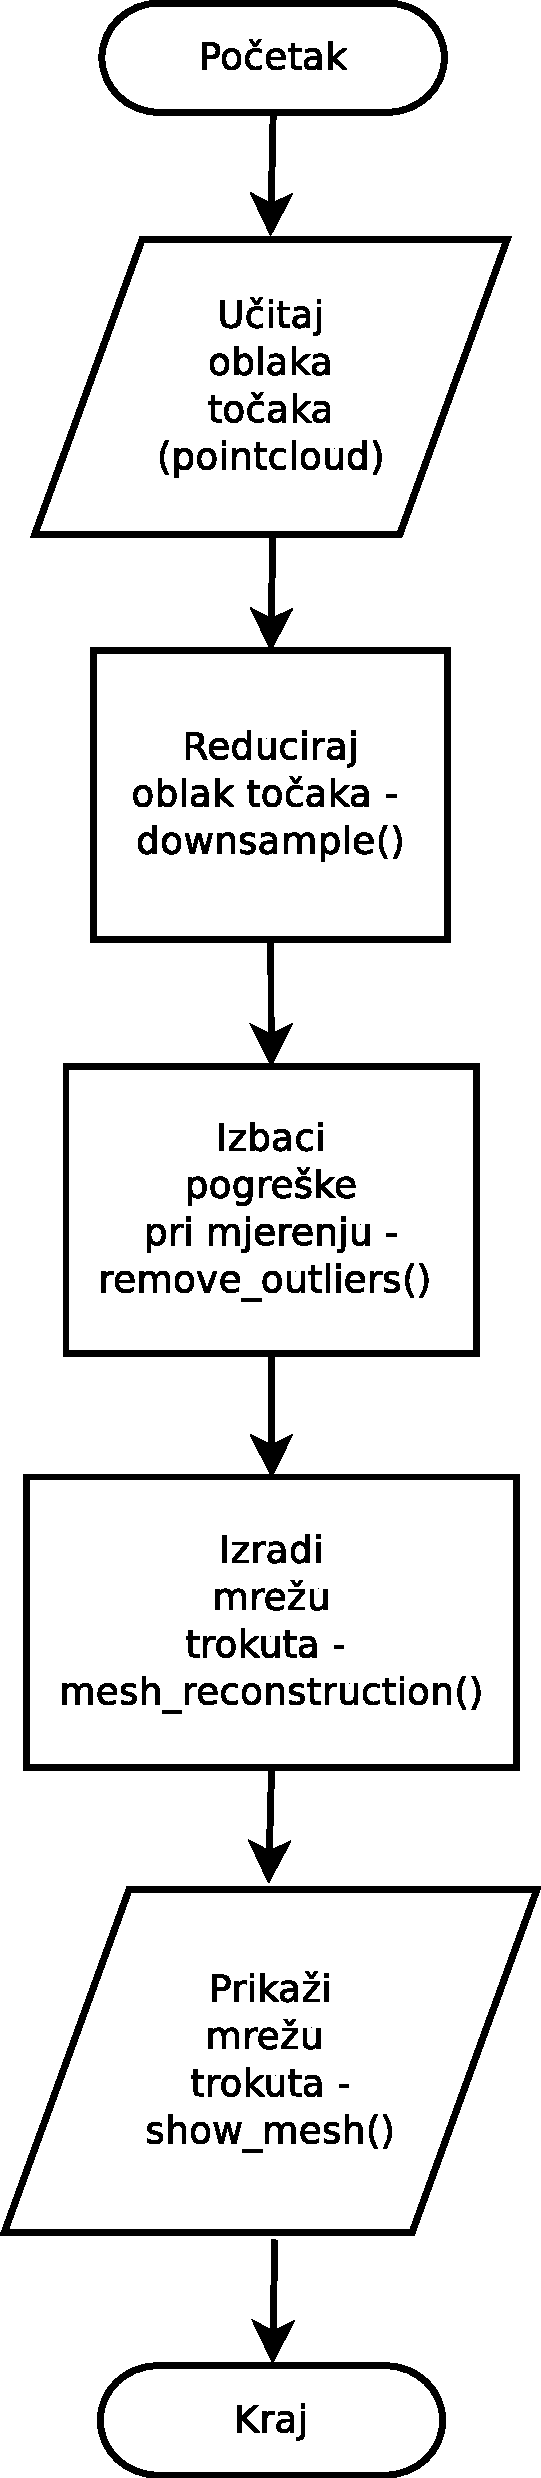
\includegraphics[scale=0.5]{figures/flowchart.pdf}
\caption{Dijagram toka programa \textit{mesh-reconstruction} }
\label{fig:flowchart}
\end{figure}

\subsubsection{Učitavanje oblaka točaka} % (fold)
\label{ssub:Učitavanje oblaka točaka}
Program učitava podatke na početku svake funkcije, te ih zapisuje na
izlazu iz funkcije kako bih prije i poslije svake operacije bio dostupan
oblak točaka.
% subsubsection Učitavanje oblaka točaka (end)

% subsection Izgradnja 3D modela scene pomoću mreže trokuta (end)

% section Izgradnja 3D modela scene (end)
